\section{Progress}
\label{sec:progress}

\begin{frame}
  \frametitle{Root Finding And Simulation Convergence}
  \begin{itemize}
  \item \textbf{Requirements:}
    \begin{itemize}
    \item Well-behaved search domain 
    \item Clear global minimum in convergence test
    \end{itemize}
  \item \textbf{Realizations:}
    \begin{itemize}
    \item With $\chi^2$ test and residual test, there are many local minima, not
      one strong global minima
    \item Beam displacement measurement has unaccounted for uncertainty
    \item BBC Rate differences caused by beam displacement, not luminosity loss,
      which was shown to be on order of 1\% previously.
    \item Allow beam displacement to vary within uncertainty, obtain better
      results.
    \end{itemize}
  \end{itemize}
\end{frame}

\begin{frame}
  \frametitle{BBC Rate, Run 360879}
  \begin{figure}
    \includegraphics[width=0.9\linewidth]{"./figures/bbc_rate_360879_labeled_steps"}
    \caption{
      Rates hint that beam displacement is not consistent. See difference
      between step 5 and 7. Small deviations in displacement have a large
      effect on the observed z-vertex profile.
    }
    \label{fig:run_360879}
  \end{figure}
\end{frame}

\section{Results From Tuning - Horizontal Scan}

\begin{frame}
  \frametitle{Step 0}
  \begin{figure}
    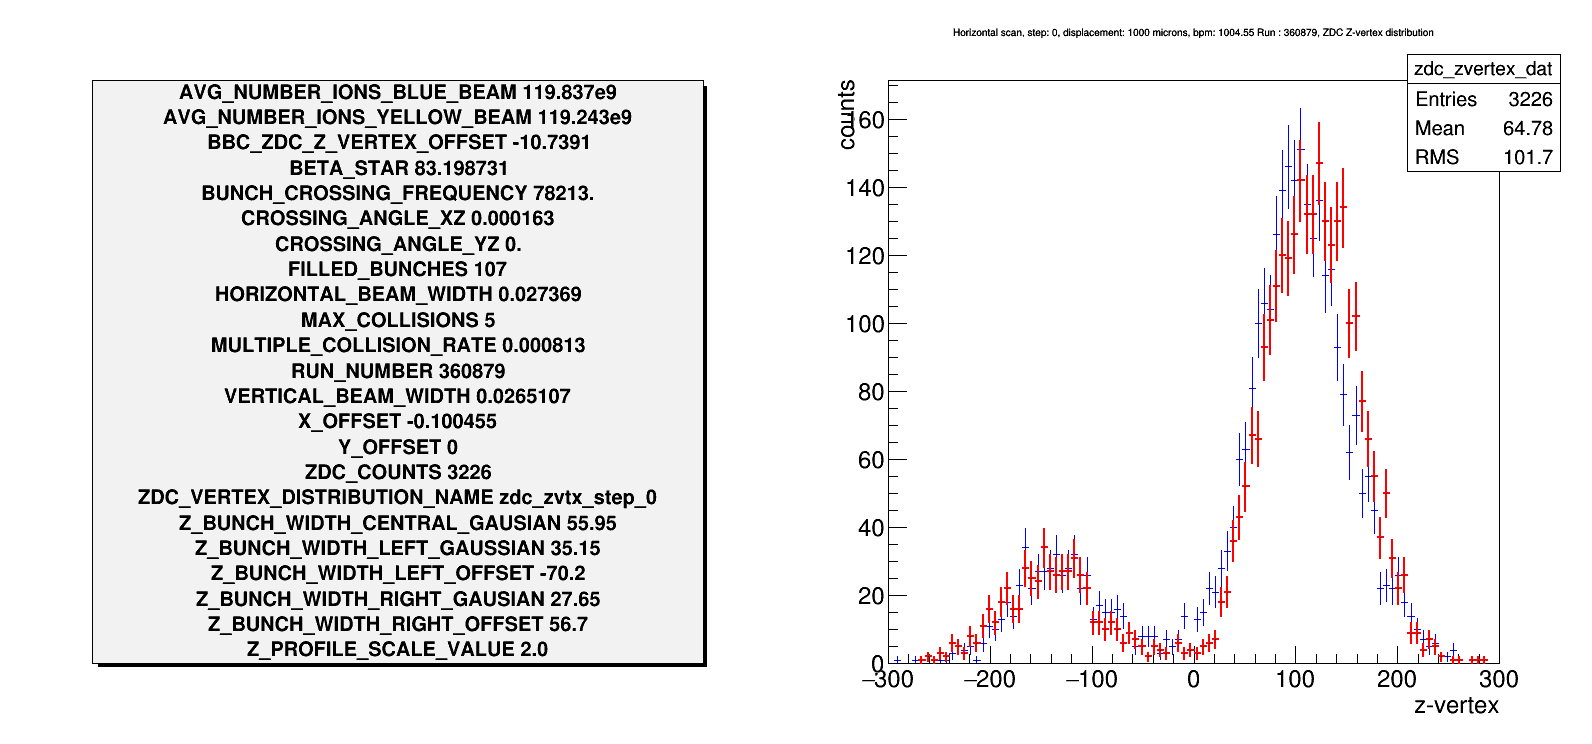
\includegraphics[width=\linewidth]{"./figures/tuned_simulation_step_0}
    \label{fig:step_0}
  \end{figure}
\end{frame}

\begin{frame}
  \frametitle{Step 1}
  \begin{figure}
    \includegraphics[width=\linewidth]{"./figures/tuned_simulation_step_1"}
    \label{fig:step_1}
  \end{figure}
\end{frame}

\begin{frame}
  \frametitle{Step 2}
  \begin{figure}
    \includegraphics[width=\linewidth]{"./figures/tuned_simulation_step_2"}
    \label{fig:step_2}
  \end{figure}
\end{frame}

\begin{frame}
  \frametitle{Step 3}
  \begin{figure}
    \includegraphics[width=\linewidth]{"./figures/tuned_simulation_step_3"}
    \label{fig:step_3}
  \end{figure}
\end{frame}

\begin{frame}
  \frametitle{Step 4}
  \begin{figure}
    \includegraphics[width=\linewidth]{"./figures/tuned_simulation_step_4"}
    \label{fig:step_4}
  \end{figure}
\end{frame}

\begin{frame}
  \frametitle{Step 5}
  \begin{figure}
    \includegraphics[width=\linewidth]{"./figures/tuned_simulation_step_5"}
    \label{fig:step_5}
  \end{figure}
\end{frame}

\begin{frame}
  \frametitle{Step 6}
  \begin{figure}
    \includegraphics[width=\linewidth]{"./figures/tuned_simulation_step_6"}
    \label{fig:step_6}
  \end{figure}
\end{frame}

\begin{frame}
  \frametitle{Step 7}
  \begin{figure}
    \includegraphics[width=\linewidth]{"./figures/tuned_simulation_step_7"}
    \label{fig:step_7}
  \end{figure}
\end{frame}

\begin{frame}
  \frametitle{Step 8}
  \begin{figure}
    \includegraphics[width=\linewidth]{"./figures/tuned_simulation_step_8"}
    \label{fig:step_8}
  \end{figure}
\end{frame}

\begin{frame}
  \frametitle{Step 9}
  \begin{figure}
    \includegraphics[width=\linewidth]{"./figures/tuned_simulation_step_9"}
    \label{fig:step_9}
  \end{figure}
\end{frame}

\begin{frame}
  \frametitle{Step 10}
  \begin{figure}
    \includegraphics[width=\linewidth]{"./figures/tuned_simulation_step_10"}
    \label{fig:step_10}
  \end{figure}
\end{frame}

\begin{frame}
  \frametitle{Step 11}
  \begin{figure}
    \includegraphics[width=\linewidth]{"./figures/tuned_simulation_step_11"}
    \label{fig:step_11}
  \end{figure}
\end{frame}

\begin{frame}
  \frametitle{Step 12}
  \begin{figure}
    \includegraphics[width=\linewidth]{"./figures/tuned_simulation_step_12"}
    \label{fig:step_12}
  \end{figure}
\end{frame}

\section{Results From Tuning - Vertical Scan}

\begin{frame}
  \frametitle{Step 13}
  \begin{figure}
    \includegraphics[width=\linewidth]{"./figures/tuned_simulation_step_13"}
    \label{fig:step_13}
  \end{figure}
\end{frame}

\begin{frame}
  \frametitle{Step 14}
  \begin{figure}
    \includegraphics[width=\linewidth]{"./figures/tuned_simulation_step_14"}
    \label{fig:step_14}
  \end{figure}
\end{frame}

\begin{frame}
  \frametitle{Step 15}
  \begin{figure}
    \includegraphics[width=\linewidth]{"./figures/tuned_simulation_step_15"}
    \label{fig:step_15}
  \end{figure}
\end{frame}

\begin{frame}
  \frametitle{Step 16}
  \begin{figure}
    \includegraphics[width=\linewidth]{"./figures/tuned_simulation_step_16"}
    \label{fig:step_16}
  \end{figure}
\end{frame}

\begin{frame}
  \frametitle{Step 17}
  \begin{figure}
    \includegraphics[width=\linewidth]{"./figures/tuned_simulation_step_17"}
    \label{fig:step_17}
  \end{figure}
\end{frame}

\begin{frame}
  \frametitle{Step 18}
  \begin{figure}
    \includegraphics[width=\linewidth]{"./figures/tuned_simulation_step_18"}
    \label{fig:step_18}
  \end{figure}
\end{frame}

\begin{frame}
  \frametitle{Step 19}
  \begin{figure}
    \includegraphics[width=\linewidth]{"./figures/tuned_simulation_step_19"}
    \label{fig:step_19}
  \end{figure}
\end{frame}

\begin{frame}
  \frametitle{Step 20}
  \begin{figure}
    \includegraphics[width=\linewidth]{"./figures/tuned_simulation_step_20"}
    \label{fig:step_20}
  \end{figure}
\end{frame}

\begin{frame}
  \frametitle{Step 21}
  \begin{figure}
    \includegraphics[width=\linewidth]{"./figures/tuned_simulation_step_21"}
    \label{fig:step_21}
  \end{figure}
\end{frame}

\begin{frame}
  \frametitle{Step 22}
  \begin{figure}
    \includegraphics[width=\linewidth]{"./figures/tuned_simulation_step_22"}
    \label{fig:step_22}
  \end{figure}
\end{frame}

\begin{frame}
  \frametitle{Step 23}
  \begin{figure}
    \includegraphics[width=\linewidth]{"./figures/tuned_simulation_step_23"}
    \label{fig:step_23}
  \end{figure}
\end{frame}

\begin{frame}
  \frametitle{Step 24}
  \begin{figure}
    \includegraphics[width=\linewidth]{"./figures/tuned_simulation_step_24"}
    \label{fig:step_24}
  \end{figure}
\end{frame}

\begin{frame}
  \frametitle{Step 25}
  \begin{figure}
    \includegraphics[width=\linewidth]{"./figures/tuned_simulation_step_25"}
    \label{fig:step_25}
  \end{figure}
\end{frame}

